\documentclass{beamer}
\usepackage[outputdir=.build]{minted}
\usemintedstyle{cevelop}
\usepackage{booktabs}
\usepackage{graphicx}
\graphicspath{{../images/}}
\usepackage{qtree}
\newcommand{\qlabelhook}{\normalsize}
\newcommand{\qleafhook}{\small\itshape}
\usetheme{metropolis}

\title{Of Owls and IO Objects}
\author{Felix Morgner}
\subtitle{OR network programming with ASIO}
\date{Oct 25, 2017}
\subject{C++ Meetup Zürich}
\institute[%
  University of Applied Sciences Rapperswil%
]{Institute for Software\\University of Applied Sciences Rapperswil}

\begin{document}
\maketitle

\section*{Introduction}

\begin{frame}
  \frametitle{What is ASIO}\pause{}
  \begin{itemize}
    \item{A type of owl}\pause{}
    \item{Audio Stream Input/Output}\pause{}
    \item{Australian Security Intelligence Organisation}\pause{}
    \item{An asynchronous I/O toolkit for C++}
  \end{itemize}
\end{frame}

\begin{frame}
  \frametitle{Why should you care}
  \begin{itemize}
    \item{Networking TS (N4656)}\pause{}
    \item{Networking is tedious}\pause{}
    \item{It's more than networking}
  \end{itemize}
\end{frame}

\begin{frame}
  \frametitle{Agenda}
  \tableofcontents
\end{frame}

\section{Software Design Patterns}

\begin{frame}
  \frametitle{Brief History}
  \begin{itemize}
    \item{Architecture: Christopher Alexander 1977/79}
      \begin{itemize}
        \item{A Place To Wait}
      \end{itemize}\pause{}
    \item{Beck \& Cunningham 1987}\pause{}
    \item{GoF Patterns (Gamma et al.) 1994}\pause{}
    \item{Many more since then}
  \end{itemize}
\end{frame}

\begin{frame}
  \frametitle{What Are Patterns}
  \begin{itemize}
    \item{Solutions to common problems}
    \item{NOT code}\pause{}
    \item{Descriptions of relevant forces}\pause{}
    \item{Language independent}
  \end{itemize}
\end{frame}

\begin{frame}
  \frametitle{Misconceptions}
  \begin{itemize}
    \item{Patterns are invented}\pause{}
    \item{GoF patterns are the only patterns}\pause{}
    \item{More patterns == Better software}\pause{}
    \item{Patterns have no drawbacks}\pause{}
    \item{Singleton is a good pattern}
  \end{itemize}
\end{frame}

\begin{frame}
  \frametitle{Pattern Sources}
  \begin{itemize}
    \item{GoF}\pause{}
    \item{POSA 1, 2, 3, 4}\pause{}
    \item{Security Patterns}\pause{}
    \item{Patterns for Fault Tolerant Software}\pause{}
    \item{Game Programming Patterns}\pause{}
    \item{Many, many more}
  \end{itemize}
\end{frame}

\begin{frame}
  \frametitle{Two Patterns for Asynchronous I/O}
  \begin{itemize}
    \item{Reactor}\pause{}
      \begin{itemize}
        \item{Notify when I/O is ready}
        \item{``Consumer'' must perform I/O}
      \end{itemize}\pause{}
    \item{Proactor}\pause{}
      \begin{itemize}
        \item{Notify when I/O is done}
        \item{``Consumer'' works with data}
      \end{itemize}\pause{}
  \end{itemize}
\end{frame}

\begin{frame}
  \frametitle{Proactor Relations}
  \vfill{}
  \begin{center}
    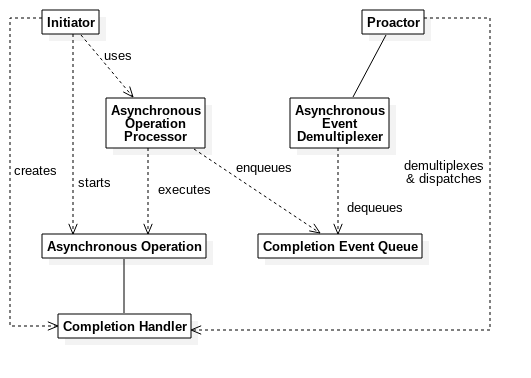
\includegraphics[width=0.8\textwidth]{proactor}
  \end{center}
\end{frame}

\section{ASIO 101}

\begin{frame}
  \frametitle{Overview}
  \begin{itemize}
    \item{Created by Christopher Kohlhoff in 2003}\pause{}
    \item{Part of the Boost libraries since 2008}\pause{}
    \item{Available on Linux, BSD, macOS, Windows, \ldots{}}\pause{}
    \item{Based on the Proactor pattern}\pause{}
    \item{NOT only for asynchronous I/O}
  \end{itemize}
\end{frame}

\begin{frame}[fragile]
  \frametitle{ASIO Hello World}
  \begin{minted}[fontsize=\footnotesize{},autogobble]{cpp}
  #include <asio.hpp>
  #include <chrono>
  #include <iostream>

  int main() {
    auto && service = asio::io_service{};
    auto && timer = asio::steady_timer{service};

    timer.expires_from_now(std::chrono::seconds{1});
    timer.async_wait([](auto error){
      std::cout << "timer fired!\n";
    });

  service.run();
  }
  \end{minted}
\end{frame}

\begin{frame}[fragile]
  \frametitle{Disecting the Example}
  \begin{itemize}
    \item{Our Proactor}
    \item{\mintinline{cpp}{service = asio::io_service{};}}\pause{}
    \item{The I/O object}
    \item{\mintinline{cpp}{timer = asio::steady_timer{service};}}\pause{}
    \item{Our asynchronous operation}
    \item{\mintinline{cpp}{timer.async_wait(...)}}\pause{}
    \item{Our completion handler}
    \item{\mintinline{cpp}{[](auto error){ ... }}}
  \end{itemize}
\end{frame}

\begin{frame}[fragile]
  \begin{centering}
    \Large{This is the basic anatomy of an ASIO program}
  \end{centering}
\end{frame}

\section{Networking}

\begin{frame}
  \frametitle{It's almost as simple}
  \begin{itemize}
    \item{OOTB Support for ICMP, TCP, UDP, IPv4/6, Multicast}\pause{}
    \item{Includes support for resolving addresses}\pause{}
    \item{Also support TLS through OpenSSL}\pause{}
    \item{``Byte-based'' and ``Condition-based''}
  \end{itemize}
\end{frame}

\begin{frame}
  \frametitle{An echo server with:}
  \begin{itemize}
    \item{N connections}\pause{}
    \item{Output queueing}\pause{}
    \item{Automatic connection lifetime}
  \end{itemize}
\end{frame}

\begin{frame}[fragile]
  \frametitle{The connection class (head)}
  \begin{minted}[fontsize=\footnotesize{}]{cpp}
  struct connection : std::enable_shared_from_this<connection> {
    // ... members
  };
  \end{minted}
\end{frame}

\begin{frame}[fragile]
  \frametitle{The connection class (data members)}
  \begin{minted}[fontsize=\footnotesize{}]{cpp}
  struct connection : ... {

  private:
    asio::ip::tcp::socket m_sock;
    asio::strand m_strand;
    std::array<char, 1024> m_buff{};
    std::deque<std::string> m_out{};
  };
  \end{minted}
\end{frame}

\begin{frame}[fragile]
  \frametitle{The connection class (ctor)}
  \begin{minted}[fontsize=\footnotesize{}]{cpp}
  struct connection : ... {

    connection(asio::ip::tcp::socket sock)
      : m_sock{std::move(sock)}
      , m_strand{m_sock.get_io_service()} {

    }

  };
  \end{minted}
\end{frame}

\begin{frame}[fragile]
  \frametitle{The connection class (starting communication)}
  \begin{minted}[fontsize=\footnotesize{}]{cpp}
  struct connection : ... {

    void start() {
      do_read();
    }

  };
  \end{minted}
\end{frame}

\begin{frame}[fragile]
  \frametitle{The connection class (reading data)}
  \begin{minted}[fontsize=\footnotesize{}]{cpp}
  struct connection : ... {

  private:
    void do_read() {
      m_sock.async_read_some(asio::buffer(m_buff),
        [&, self = shared_from_this()](auto error, auto read) {
        if(!error) {
          auto begin = m_buff.data();
          auto end = begin + read;
          m_strand.post([&, data=std::string{begin, end}]{
            write(data);
          });
        do_read();
        }
      });
    }
  };
  \end{minted}
\end{frame}

\begin{frame}[fragile]
  \frametitle{The connection class (writing data part 1)}
  \begin{minted}[fontsize=\footnotesize{}]{cpp}
  struct connection : ... {

  private:
    void write(std::string data) {
      m_out.push_back(data);

      if(m_out.size() < 2) {
        do_write();
      }
    }
  };
  \end{minted}
\end{frame}

\begin{frame}[fragile]
  \frametitle{The connection class (writing data part 2)}
  \begin{minted}[fontsize=\footnotesize{}]{cpp}
  struct connection : ... {

  private:
    void do_write() {
      asio::async_write(m_sock, asio::buffer(m_out.front()),
        m_strand.wrap([&, self = shared_from_this()](auto error,
                                                    auto written) {
        m_out.pop_front();

        if(!error) {
          if(!m_out.empty()) {
            do_write();
          }
        }
      }));
    }
  };
  \end{minted}
\end{frame}

\begin{frame}
  \frametitle{Review of the connection class}
  Connections:\pause{}
  \begin{itemize}
    \item{keep themselves alive}\pause{}
    \item{have a single input buffer}\pause{}
    \item{have an output queue}
  \end{itemize}
\end{frame}

\begin{frame}[fragile]
  \frametitle{The server class (data members)}
  \begin{minted}[fontsize=\footnotesize{}]{cpp}
  struct server {

  private:
     asio::ip::tcp::acceptor m_acceptor;
     asio::ip::tcp::socket m_sock;
  };
  \end{minted}
\end{frame}

\begin{frame}[fragile]
  \frametitle{The server class (creation)}
  \begin{minted}[fontsize=\footnotesize{}]{cpp}
  struct server {

  server(asio::io_service & service)
    : m_acceptor{service,
                 asio::ip::tcp::endpoint{
                   asio::ip::tcp::v4(),
                   4321}}
    , m_sock{service} {}

  };
  \end{minted}
\end{frame}

\begin{frame}[fragile]
  \frametitle{The server class (starting)}
  \begin{minted}[fontsize=\footnotesize{}]{cpp}
  struct server {

  void start() {
    do_accept();
  }

  };
  \end{minted}
\end{frame}

\begin{frame}[fragile]
  \frametitle{The server class (accepting connections)}
  \begin{minted}[fontsize=\footnotesize{}]{cpp}
  struct server {

  private:
    void do_accept() {
      m_acceptor.async_accept(m_sock, [&](auto error){
        if(!error) {
          auto conn = std::make_shared<connection>(
            std::move(m_sock)
          );
          conn->start();
          do_accept();
        }
      });
    }
  };
  \end{minted}
\end{frame}

\begin{frame}
  \frametitle{Review of the server class}
  Our server:\pause{}
  \begin{itemize}
    \item{accepts new connections}\pause{}
    \item{creates \mintinline{cpp}{connection} objects}\pause{}
    \item{does not care about the connections}
  \end{itemize}
\end{frame}

\begin{frame}[fragile]
  \frametitle{Glueing it all together}
  \begin{minted}[fontsize=\footnotesize{}]{cpp}
    auto && service = asio::io_service{};
    auto && server = ::server{service};

    server.start();
  \end{minted}
\end{frame}

\begin{frame}[fragile]
  \frametitle{Glueing it all together (contd.)}
  \begin{minted}[fontsize=\footnotesize{}]{cpp}
    service.run();
  \end{minted}
\end{frame}

\begin{frame}[fragile]
  \frametitle{Glueing it all together (contd.)}
  \begin{minted}[fontsize=\footnotesize{}]{cpp}
    auto const cpus = std::thread::hardware_concurrency();
    auto pool = std::vector<std::future<void>>{cpus};

    for(auto & future : pool) {
      future = std::async(std::launch::async, [&]{
        service.run();
      });
    }
  \end{minted}
\end{frame}

\begin{frame}
  \begin{center}
    \Huge{Demo Time!}
  \end{center}
\end{frame}

\begin{frame}
  \frametitle{There is more}
  \begin{itemize}
    \item{stream buffers}\pause{}
    \item{conditions}\pause{}
    \item{TLS}\pause{}
    \item{Name resolution}\pause{}
    \item{Synchronous I/O}
  \end{itemize}
\end{frame}

\section{Beyond Networking}

\begin{frame}
  \frametitle{It's More Than Networking}\pause{}
  \begin{itemize}
    \item{Signal handling}\pause{}
    \item{General worker pool}\pause{}
    \item{Stream I/O}\pause{}
    \item{Serial ports}\pause{}
    \item{Timers}\pause{}
    \item{File I/O (Windows)}
  \end{itemize}
\end{frame}

\begin{frame}[fragile]
  \frametitle{Signal handling}
  \begin{minted}[fontsize=\footnotesize{}]{cpp}
  auto && signals = asio::signal_set(service, SIGINT);
  signals.add(SIGINT);
  signals.async_wait([&](auto error, auto signal){
    if(!error && !service.stopped()) {
      std::cout << "Received SIGINT. Terminating. " << '\n';
      service.stop();
    }
  });
  \end{minted}
\end{frame}

\begin{frame}[fragile]
  \frametitle{Worker Pool (posting the work)}
  \begin{minted}[fontsize=\footnotesize{}]{cpp}
    service.post([&]{
      prove_p_equals_np();
    });
  \end{minted}
\end{frame}

\begin{frame}[fragile]
  \frametitle{Worker Pool (posting the work)}
  \begin{minted}[fontsize=\footnotesize{}]{cpp}
    service.post([&]{
      factor_large_rsa_key();
    });
  \end{minted}
\end{frame}

\begin{frame}[fragile]
  \frametitle{Worker Pool (posting the work)}
  \begin{minted}[fontsize=\footnotesize{}]{cpp}
    service.post([&]{
      invent_time_machine();
    });
  \end{minted}
\end{frame}

\begin{frame}[fragile]
  \frametitle{Worker Pool (posting the work)}
  \begin{minted}[fontsize=\footnotesize{}]{cpp}
    service.post([&]{
      std::do_stuff();
    });
  \end{minted}
\end{frame}

\begin{frame}[fragile]
  \frametitle{Worker Pool (running the workers)}
  \begin{minted}[fontsize=\footnotesize{}]{cpp}
    auto const cpus = std::thread::hardware_concurrency();
    auto pool = std::vector<std::future<void>>{cpus};

    for(auto & future : pool) {
      future = std::async(std::launch::async, [&]{
        service.run();
      });
    }
  \end{minted}
\end{frame}


\section{Summary and Q\&A}
\begin{frame}
  \frametitle{Conclusion}
  \begin{itemize}
    \item{ASIO is not a framework!}\pause{}
    \item{It is not that scary}\pause{}
    \item{Provides rich I/O and event handling}\pause{}
    \item{Parts of it will be standard C++}
  \end{itemize}
\end{frame}
\begin{frame}
  \begin{center}
    \Huge{Questions?}
  \end{center}
\end{frame}
\end{document}
